\documentclass[3pt,landscape]{article}
%ss[10pt,landscape]{article}
\usepackage{multicol}
\usepackage{calc}
\usepackage{ifthen}
\usepackage[landscape]{geometry}
\usepackage{amsmath,amsthm,amsfonts,amssymb}
\usepackage{color,graphicx,overpic}
\usepackage{hyperref}


\pdfinfo{
/Title (example.pdf)
/Creator (TeX)
/Producer (pdfTeX 1.40.0)
/Author (Seamus)
/Subject (Example)
/Keywords (pdflatex, latex,pdftex,tex)}

% This sets page margins to .5 inch if using letter paper, and to 1cm
% if using A4 paper. (This probably isn't strictly necessary.)
% If using another size paper, use default 1cm margins.
\ifthenelse{\lengthtest { \paperwidth = 11in}}
    { \geometry{top=.3in,left=.3in,right=.3in,bottom=.3in} }
    {\ifthenelse{ \lengthtest{ \paperwidth = 297mm}}
        {\geometry{top=1cm,left=1cm,right=1cm,bottom=1cm} }
        {\geometry{top=1cm,left=1cm,right=1cm,bottom=1cm} }
    }

% Turn off header and footer
\pagestyle{empty}

% Redefine section commands to use less space
\makeatletter
\renewcommand{\section}{\@startsection{section}{1}{0mm}%
                            {-1ex plus -.5ex minus -.2ex}%
                            {0.5ex plus .2ex}%x
                            {\normalfont\large\bfseries}}
\renewcommand{\subsection}{\@startsection{subsection}{2}{0mm}%
                            {-1explus -.5ex minus -.2ex}%
                            {0.5ex plus .2ex}%
                            {\normalfont\normalsize\bfseries}}
\renewcommand{\subsubsection}{\@startsection{subsubsection}{3}{0mm}%
                            {-1ex plus -.5ex minus -.2ex}%
                            {1ex plus .2ex}%
                            {\normalfont\small\bfseries}}
\makeatother

% Define BibTeX command
\def\BibTeX{{\rm B\kern-.05em{\sc i\kern-.025em b}\kern-.08em
    T\kern-.1667em\lower.7ex\hbox{E}\kern-.125emX}}

% Don't print section numbers
\setcounter{secnumdepth}{0}


\setlength{\parindent}{0pt}
\setlength{\parskip}{0pt plus 0.5ex}

%My Environments
\newtheorem{example}[section]{Example}
% -----------------------------------------------------------------------

\def\ci{\perp\!\!\!\perp}

\begin{document}
\raggedright
\footnotesize
\begin{multicols}{3}


% multicol parameters
% These lengths are set only within the two main columns
%\setlength{\columnseprule}{0.25pt}
\setlength{\premulticols}{1pt}
\setlength{\postmulticols}{1pt}
\setlength{\multicolsep}{1pt}
\setlength{\columnsep}{2pt}

\begin{center}
    \Large{\underline{CS 161 Final Note Sheet}} \\
\end{center}

\subsubsection*{Kerchoff's Principle}
You should not rely on the secrecy of the algorithm/protocol and or keysize, as wall as the possible plain text for security because eventually the adversary will figure them out.

\subsubsection*{Mono-Alphabetic Ciphers: 1 to 1 mapping of characters to symbols}
\begin{itemize}
    \item Subsitution
        \begin{itemize}
            \item Shift or Caesar's Cipher
                \(E_{k}(m) \leftarrow m+k(\texttt{mod } N)\)
                \(D_{k}(c) \leftarrow c-k(\texttt{mod } N)\)
            \item Affine Cipher:
                \(E_{k}(m) \leftarrow k_{!}m+k_{2}(\texttt{mod } N)\)
                \(D_{k}(c) \leftarrow k_{!}^{-1}(c-k(\texttt{mod } N)\)
            \item Substitution Ciphers have an extreme vulnerability to frequency attacks.
        \end{itemize}
\end{itemize}

\subsubsection*{Poly-Alphabetic Ciphers}
\begin{itemize}
    \item Vigenere Cipher: Shift by a repeated key
    \item Book Cipher (Beale Cipher) key is hidded in a passage of a set book.
    \item Vernam Cipher
        \begin{itemize}
            \item Message is m bits and the key is n bits.
            \item Bitwise xor the message and the key, if m is greater than n, then use the key multiple times.
        \end{itemize}
    \item One-Time Pad
        \begin{itemize}
            \item Same idea as the Vernam Cipher except we use a key that is the same length or greater than the length of the message, then discard it after each use.
        \end{itemize}
    \item Transposition/Permutation Cipher
        \begin{itemize}
            \item Break the message into n bit blocks, then on each block perfom the same permutation
            \item Despite being polyalphabit, the cipher is still vulnerable to frequency attacks. Because the original patterns are still basically present. You can attack by checking anagrams.
        \end{itemize}
\end{itemize}

\subsection*{Data Encryption Standard (DES)}
DES is a block cipher in which messages are divided into data blocks of a fixed length and each block is treated as one message either in M or in C. The DES encryping and decryption algorithms take as an input a 64-bit plaintext or ciphertext message and a 56-bit key, and output a 64-bit ciphertext or plaintext message.
DES is done in 3 steps:
\begin{enumerate}
    \item Apply a fixed "initial permutation" IP to the input block.
        \((L_0,R_0) \leftarrow IP(\texttt{Input Block})\) 
        This step has no apparent cryptographic significance.
    \item Iterate the following 16 rounds of operations (Feistel Cipher)\\
        \begin{center}
        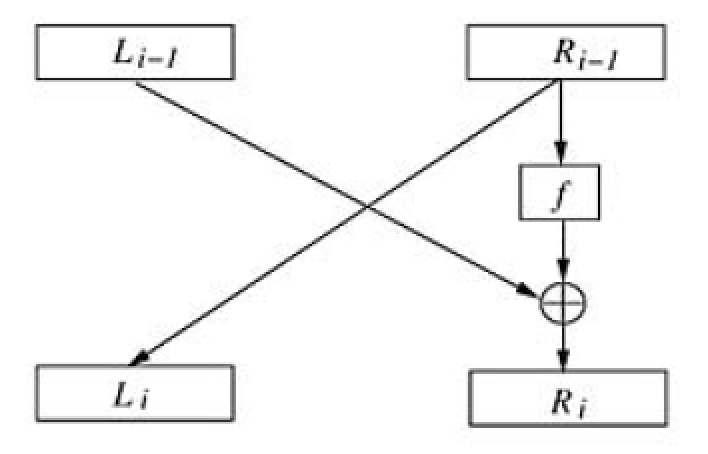
\includegraphics[scale=.47]{feistel}
        \end{center}
        \begin{itemize}
            \item the function is nonlinear and is considered a Substitution Cipher
            \item the move from \(L_{i} \rightarrow R_{i-1}\) is a Transposition cipher
            \item Vernam cipher is used at the xor
            \item k is a 48 bit subsection of the 56 bit, "round key"
        \end{itemize}
\end{enumerate}

\subsubsection*{Single DES}
\begin{itemize}
    \item vulnerable to brute force or exaustive key search attacks
\end{itemize}

\subsubsection*{Triple DES}
Triple DES uses an encryption-decryption-encryption scheme,\\
\(c \leftarrow E_{k_{1}}(D_{k_{2}}(E_{k_{1}}(m)))\)\\
\(m \leftarrow D_{k_{1}}(E_{k_{2}}(D_{k_{1}}(m)))\)\\
This scheme enlarges the keyspace while maintaining backward compatibility with single DES if \(k_{1}=k_{2}\)\\

\subsection*{Advanced Encryption Standard (AES)}
AES is a block cipher with variable block size and variable keysize. (block size can be 128, 192, 256 bit)\\
AES has 4 states:
\begin{enumerate}
    \item Sub Bytes State: nonlinear substitution on each byte
    \item Shift Rows State: Transposition rearranges the order of elements in each row
    \item Mix Columns State: Polynomial multiplication after converting column to polynomial.
    \item Add Round Key State: adds elements of round key to the state, basically bitwise "OR"
\end{enumerate}
Decryption is the inverse of these steps.

\subsubsection*{Confidentiality Modes of Operation}
Different modes of operation have been devised on top of an underlying block cipher algorithm
\begin{itemize}
    \item Electronic Codebook (ECB) Mode
        This mode encrypts and decrypts every block seperately. It is deterministic and leaves patterns in the cipher text. (for example images.)
    \item Cipher Block Chaining (CBC) Mode
        \begin{itemize}
            \item This is the most common mode of operation. In this mode the output is a sequence of n-bit cipher blocks which are chained together so that each cipher block is dependent on all the previous data blocks.
            \item Decryption can be done in parallel
            \item CBC cannot prived data integrity protection.
            \item If the CBC claims data integrity protection, Eve can use (Bomb Oracle Attack) a Decryption Oracle to figure out the padding scheme and eventually the last byte of the cipher text.
        \end{itemize}
\end{itemize}
\begin{center}
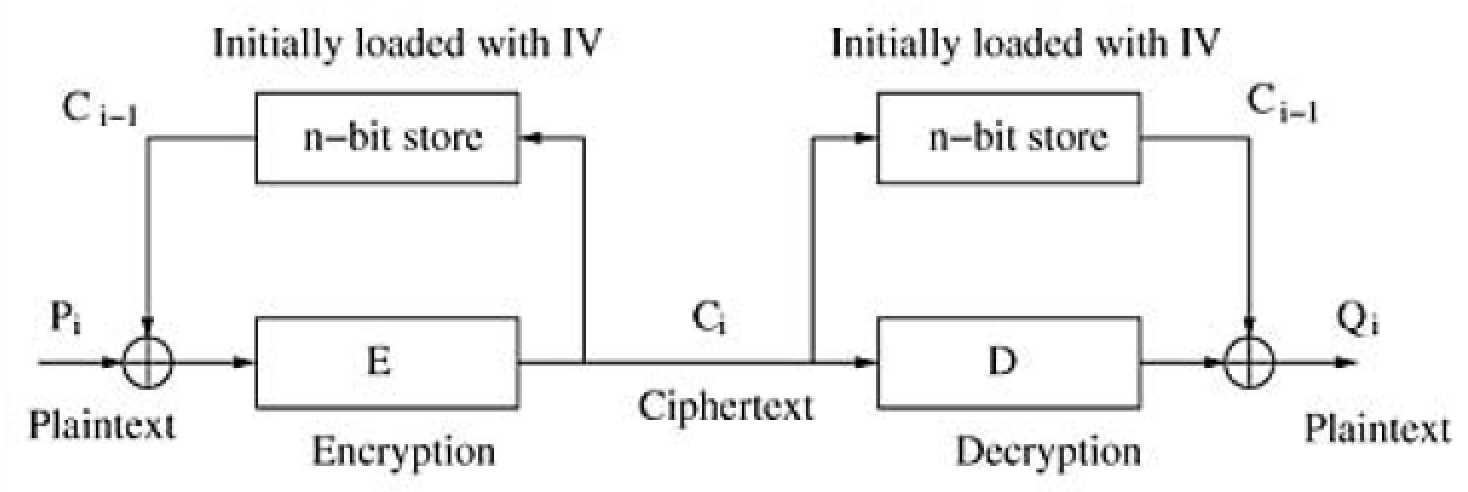
\includegraphics[scale=.33]{CBCMode}
\end{center}
\begin{itemize}
    \item Cipher Feedback (CFB) Mode
        \begin{itemize}
            \item CFB mode of opration features feeding successive cipher segments which are output from the mode back as input to the underlying block cipher algorithm.
            \item CFB requires an IV as the initial n-bit input block
        \end{itemize}
\end{itemize}
\begin{center}
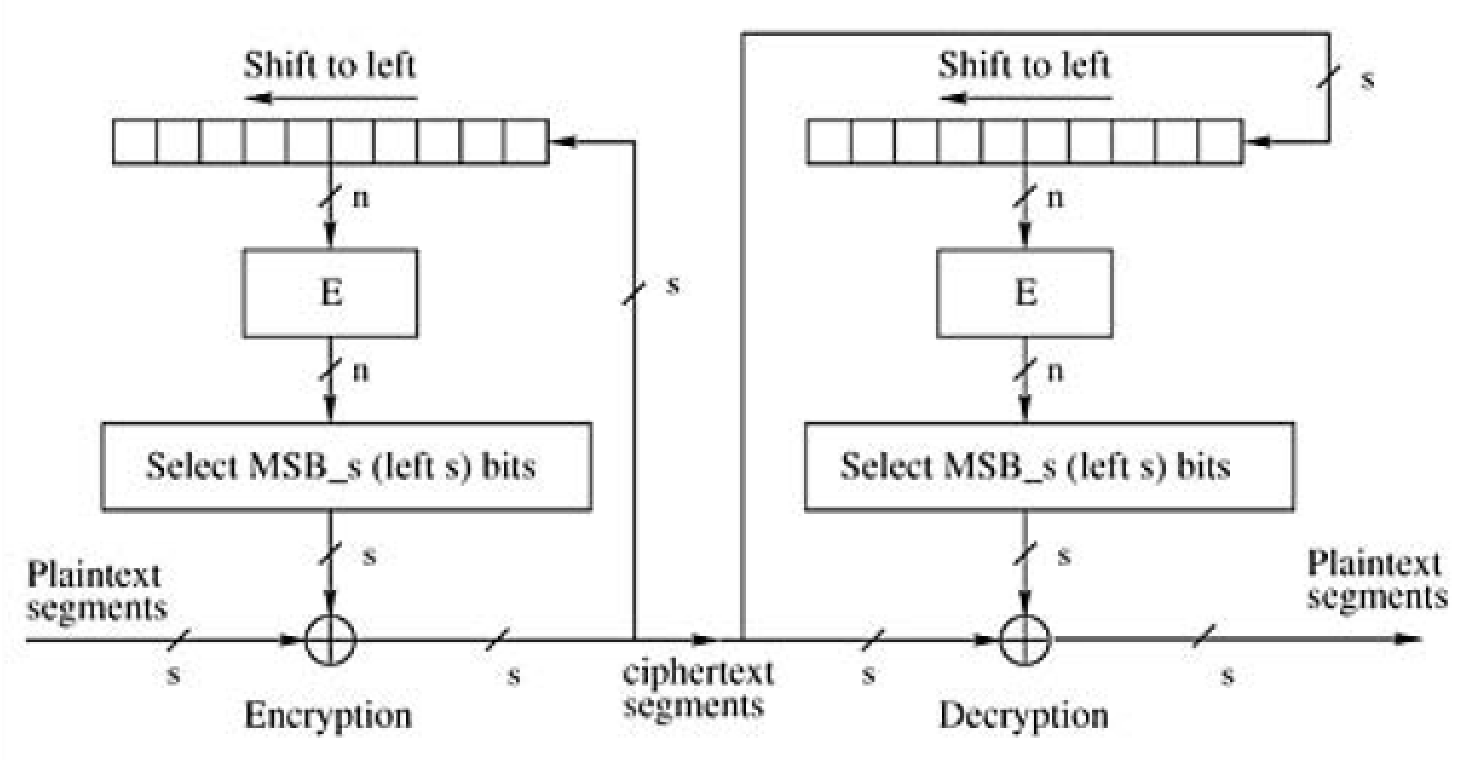
\includegraphics[scale=.35]{CFBMode}
\end{center}
\begin{itemize}
    \item Output Feedback (OFB) Mode
        \begin{itemize}
            \item The OFB mode feeds successive output blocks from the underlying block cipher back to it.
            \item The feedback blocks form a string of bits which used as the key stream of the Vernam cipher.
        \end{itemize}
\end{itemize}
\begin{center}
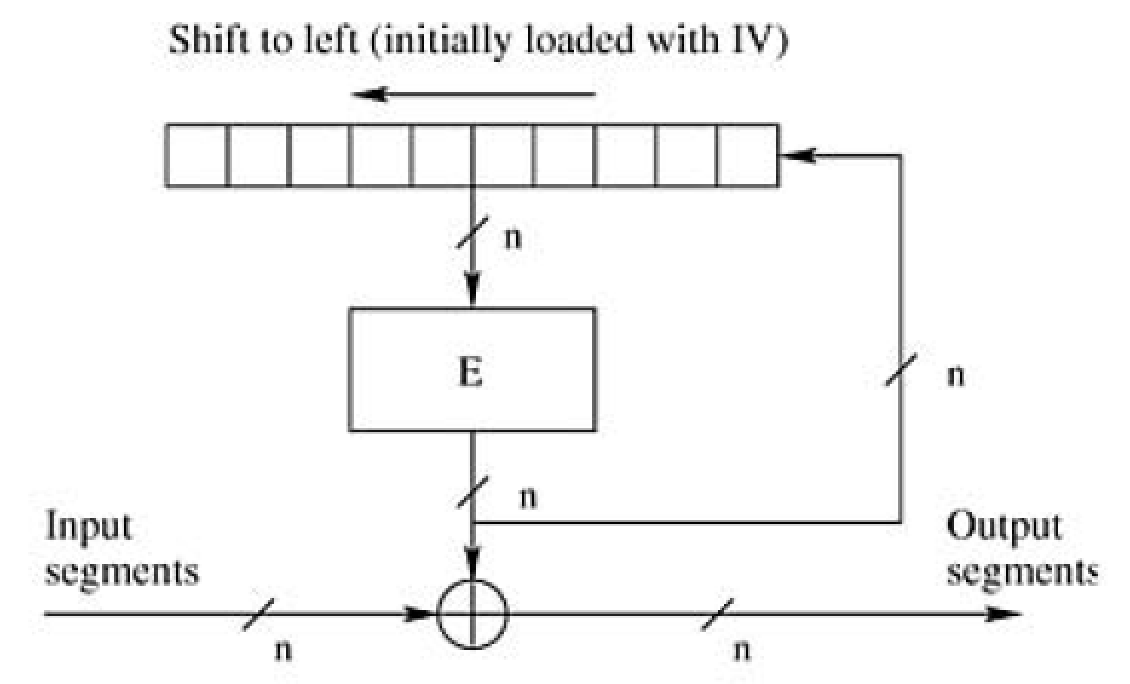
\includegraphics[scale=.32]{OFBMode}
\end{center}
\newpage
\begin{itemize}
    \item Counter (CTR) Mode
        \begin{itemize}
            \item The CTR mode features feeding the underlying block cipher algorithm with a counter value which counts up from an initial value. With a counter counting up, the underlying block cipher algorithm outputs successive blocks to form a string of bits. This string of bits is used as the key stream of the vernam cipher, that is, the key stream is XOR-ed with the plaintext blocks.
                \(C_{i} \leftarrow P_{i} \oplus E(Ctr_{i}, i=1,2,\ldots,m\)\\
                \(P_{i} \leftarrow C_{i} \oplus E(Ctr_{i}, i=1,2,\ldots,m\)
        \end{itemize}
\end{itemize}

\subsubsection*{Bomb Oracle Attack}
% todo

\subsection*{Asymmetric Cryptography}
\subsubsection*{Oneway Trapdoor Function}
\begin{itemize}
    \item Asymmetric crypto system, Public Key Cryptography
    \item \(D \rightarrow R\) is oneway, it is easy to evaluate \(\forall x \in D\) and difficult to invert for all values in R.
\end{itemize}

\subsubsection*{Textbook Encryption Algorithms}
\begin{itemize}
    \item All or Nothing Secrecy: Given Cipher Text the attacker must not be able to get any information about the plain text
    \item Passive Attacker: The attacker doesn't modify or manipulate ciphertexts they also don't ask for encryption or Decryption services. % todo check definition and move to it's own section
\end{itemize}

\subsection*{Diffie-Hellman Key Exchange Protocol}
\(\begin{array}{ll}
    \texttt{Common Input} & (p,g):p \texttt{ is a large prime, g is a generator}\\
    \texttt{ } & \texttt{element in } F_{p}^{*}\\
    \texttt{Output} & \texttt{An element in } F_{p}^{*} \texttt{ shared between Alice}\\
    \texttt{ } & \texttt{Bob.}
\end{array}\)
\begin{enumerate}
    \item Alice picks \(a \in U(1,p-1)\); computes \(g_{a} \leftarrow g^{a}(\texttt{mod } p)\); sends \(g_{a}\) to Bob.
    \item Bob picks \(b \in U(1,p-1)\); computes \(g_{b} \leftarrow g^{b}(\texttt{mod } p)\); sends \(g_{b}\) to Alice.
    \item Alice computes \(k \leftarrow g_{b}^{a}(\texttt{mod } p)\)
    \item Bob computes \(k \leftarrow g_{a}^{b}(\texttt{mod } p)\)
\end{enumerate}
Alice and Bob both compute the same key,
\[k = g^{ba}(\texttt{mod }p) = g^{ab}(\texttt{mod }p)\]
P is a public 2048 bit prime number.

\subsubsection*{Man in the Middle Attack on Diffie-Helman}
\begin{center}
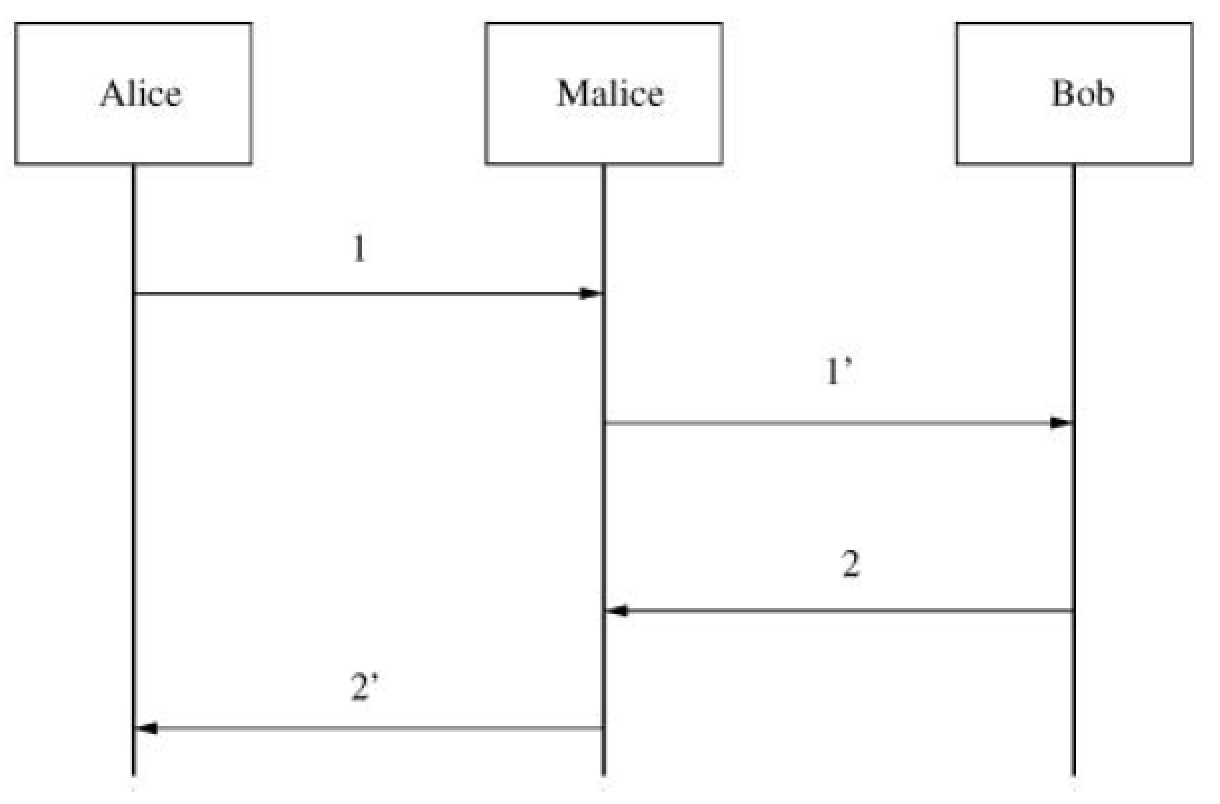
\includegraphics[scale=.26]{DiffieHelmanMITM}
\end{center}
\begin{enumerate}
    \item Alice picks a \(\in _{u}[1,p-1)\), computes \(g_{a} \leftarrow g^{a}(\texttt{mod }p)\) she sends \(g_{a}\) to Malice("bob");
    \item (1') Malice("Alice") computes \(g_{m} \leftarrow g^{m}(\texttt{mod })\) for some \(m \in [1,p-1)\); he sends \(g_{m}\) to Bob;
    \item (2) Bob picks \(b \in _{U}[1,p-1)\), computes \(g_{b} \leftarrow g^{b}(\texttt{mod }p)\); he sends \(g_{b}\) Malice("Alice");
        \item (2') Malice("Bob") sends to Alice: \(g_{m}\);
        \item (3) Alice computes \(k_{1} \leftarrow g^{a}_{m}(\texttt{mod }p)\);
        \item (4) Bob computes \(k_{2} \leftarrow g^{b}_{m}(\texttt{mod }p)\);
\end{enumerate}

\subsubsection*{Diffie-Helman and the Discrete Logarithm Problem}
\begin{itemize}
    \item Computational Diffie-Hellman (CDH) Problem
        \(\begin{array}{ll}
            \texttt{INPUT} & \texttt{desc}(F_{q}): \texttt{a finite field } F_{q}\\
            \texttt{ } & g^{a},g^{b} \in F^{*}_{q} \texttt{for some integers } 0<a,b<q\\
            \texttt{OUTPUT} & g^{ab}
        \end{array}\)
    \item Discrete Logarithm Problem
        \(\begin{array}{ll}
            \texttt{INPUT} & \texttt{desc}(F_{q}): \texttt{a finite field } F_{q}\\
            \texttt{ } & g \in F_{q}^{*}\\
            \texttt{ } & h \in F_{q}^{*}\\
            \texttt{OUTPUT} & \texttt{the unique integer } (a<q) \texttt{ such that } h = g^{a}
        \end{array}\)
\end{itemize}
If the Discrete Logarithm Problem is solved, then the CDH Problem is also solved. But not necessarily vice versa.

\subsubsection*{Eulers Theorem}
given a,n are coprime,\\
\(a^{\phi(n)}=1(\texttt{mod }n)\)

\subsubsection*{Fermat's Little Theorem}
given a coprime to N,\\
\(a^{(N-1)}=1(\texttt{mod }N)\), \(a \in \mathbb{Z}<N\)

\subsection*{Cryptanalysis Against Public-key Cryptosystems}
\subsubsection*{Chosen-Plain Text Attack (CPA)}
\begin{itemize}
    \item An attack chooses a plaintext messages and gets encryption assistance to obtain the corresponding ciphertext messages. The task for the attacker is to weaken the targeted cryptosystem using the obtained plain-text pairs.
    \item The attacker has an encryption box.
    \item All public key encryption systems must resist CPA otherwise it is useless.
\end{itemize}

\subsubsection*{Chosen-Ciphertext Attack (CCA)}
\begin{itemize}
    \item An attacker chooses ciphertext messages and gets decryption assistance to obtain the corresponding plaintext messages. The task for the attacker is to weaken the targeted cryptosystem using the obtained plaintext-ciphertext pairs. The attacker is successful if he can retrieve some secret plaintext information from a "target ciphertext" which is given to the attacker after the decryption assistance is stopped. That is, upon the attacker receipt of the target ciphertext, the decryption assistance is no longer available.
    \item The attacker is entitled to a conditional use of a decryption box. The box turns off before the ciphertext is sent.
\end{itemize}

\subsubsection*{Adaptive Chosen-Ciphertext Attack (CCA2)}
\begin{itemize}
    \item This is a CCA where the decryption assistance for the targeted cryptosystem will be available forever, except for the target ciphertext.
    \item The attacker has the decryption box for as long as he wishes, except they can't decipher the original message.
\end{itemize}

\subsubsection*{RSA Cryptosystem}
\begin{itemize}
    \item Key Setup
    \begin{enumerate}
        \item Choose two random prime numbers p and q (typically done by applyling a Monte-Carlo prime number finding algorithm.
        \item Compute \(N=pq\)
        \item Compute \(\phi(N) = (p-1)(q-1)\)
        \item Choose a random integer \(e < \phi(N)\) such that gcd\((e,\phi(n))=1\), and compute the integer d, such that,
            \[ed \equiv 1 (\texttt{mod }\phi(N))\]
        \item Publicize (N,e) as the public key, safely destroy p, q, and \(\phi(N)\), and keep d as the private key.
    \end{enumerate}
    \item Encryption\\
    To send a confidential message \(m<N\) to Alice, the sender Bob creates the ciphertext c as follows,
        \[c \leftarrow m^{e}(\texttt{mod }N)\]
    \item Decryption\\
    To decrypt the ciphertext c, Alice computes,
        \[m \leftarrow c^{d}(\texttt{mod }N)\]
\end{itemize}

\subsubsection*{Proof of RSA}
\(m = (m^{e})^{d} \texttt{mod } N\)\\
\(m = m^{e^{d}}\texttt{mod }N \texttt{, because } ed=1\texttt{mod } \phi(N)\)\\
\(ed = a+k\phi(N)\)\\
\(m = m^{1+k\phi(N)}\texttt{mod }N\)\\
\(m = m(m^{\phi(N)})^{k}\texttt{mod }N\)\\
\(m = m(\texttt{mod }N), \texttt{ iff } gcd(m,N)=1\)

\subsubsection*{RSA Problem and the Integer Factorization Problem}
\begin{itemize}
    \item The RSA Problem
        \(\begin{array}{ll}
            \texttt{INPUT} & N=pq \texttt{with } p,q \texttt{ prime numbers}\\
            \texttt{ } & e \texttt{: and integer such that,}\\
            \texttt{ } & \texttt{ } gcd(e, (p-1)(q-1)) = 1\\
            \texttt{ } & c \in Z^{*}_{N}\\
            \texttt{OUTPUT} & \texttt{the unique integer } m \in Z^{*}_{N} \texttt{ satisfying,}\\
            \texttt{ } & \texttt{ } m^{e} \equiv c(\texttt{mod }N)
        \end{array}\)
    \item The Integer Factorization Problem
        \(\begin{array}{ll}
            \texttt{INPUT} & N \texttt{: odd composite integer with at least two}\\
            \texttt{ } & \texttt{distict prime factors.}\\
            \texttt{OUTPUT} & \texttt{prime p such that } p|N\\
        \end{array}\)
    \item The difficulty of the RSA problem depends, in turn, on the difficulty of the integer factorization problem.
\end{itemize}

\subsubsection*{RSA Euler's Theorem}
\(m^{p-1)(q-1)} \equiv 1(\texttt{mod }pq)\)

\subsubsection*{Insecurity of Textbook RSA Encryption}
\begin{itemize}
    \item The RSA Cryptosystem is "all-or-nothing" secure against CPA if and only if the RSA assumption holds, meaning if the attacker has some prior knowledge of the contents of a message (ex a number or bid), they may be able to successfully bruteforce a solution.\\
        \vspace{2 mm}
        For a plaintext m (\textless N), with a non-negligible probability, only \(\sqrt{m}\) trials are needed to pinpoint m if \(\sqrt{m}\) size of memory is available, exploiting,
        \[(m_{1}\cdot m_{2})^{e} \equiv m_{1}^{e} \cdot m_{2}^{e} (\texttt{mod }N)\]
    \item Let \(c = m^{e}(\texttt{mod N})\) such that Malice knows \(m<2\). With non-negligible probability m is a composite number satisfying,
        \[m = m_{1} \cdot m_{2} \texttt{ with } m_{1},m_{2} < 2^{\frac{l}{2}}\]
        and with RSA's multiplicative property, we have,
        \[c = m_{1}^{e} \cdot m_{2}^{e}(\texttt{mod }N)\]
        Malice can build a sorted database
        \[\{1^{e},2^{e},\ldots,(2^{\frac{l}{2}})^{e}\}(\texttt{mod }N)\]
        Then they can search through the sorted database trying to find \(c/i^{e}(\texttt{mod }N)\) for \(i=1,2,\ldots,2^{\frac{l}{2}}\) a finding signaled by,
        \[c/i^{e} \equiv j^{e}(\texttt{mod }N)\]
        Acheiving a square-root level reduction in time complexity.
    \item Let Malice be in conditional control of Alice's RSA decryption box. If the ciphertext submitted by Malice is not meaningful, then Alice should return the plaintext to Malice. This is reasonable because of the following:
        \begin{enumerate}
            \item "A random response for a random challenge" is a standard mode of operation in many cryptographic protocols. (including in the Needham-Schroeder protocol)
            \item This random-looking decryption result should not provide an attacker with any useful information.
        \end{enumerate}
        Malice wants to know the plaintext of a ciphertext \(c \equiv m^{e}(\texttt{mod }N)\) which he has eavesdropped.\\
        \vspace{2 mm}
        He picks a random number, \(r \in Z^{*}_{N}\), and computes \(c'=r^{e}c(\texttt{mod }N)\) and sends his chosen cipher text, c', to Alice. Alice will return,
        \[c'^{d} \equiv rm(\texttt{mod }N)\]
        Which will appear completely random to Alice.\\
        Then because Malice has r, he can obtain m with a division modulo N.
\end{itemize}

\subsection*{Data Integrity}
Data Integrity is the security service against unauthorized modification of messages.
\subsubsection*{Manipulation Detection Codes (MDC)}
\begin{itemize}
    \item Let \(K_{e}\) denote an encoding key and \(K_{v}\) denote a verification key which matches the encoding key.\\
    \item Manipulation Detection Code creation:
        \[\texttt{MDC} \leftarrow f(K_{e},\texttt{Data})\]
    \item Manipulation Detection Code verification:
        \[g(K_{v},\texttt{Data},\texttt{MDC})
        =\left\{\begin{array}{ll}
                \texttt{True} & \texttt{if MDC}=f(K_{e},\texttt{Data})\\
                \texttt{False} & \texttt{if MDC}\neq f(K_{e},\texttt{Data})
            \end{array}\right.\]
\end{itemize}
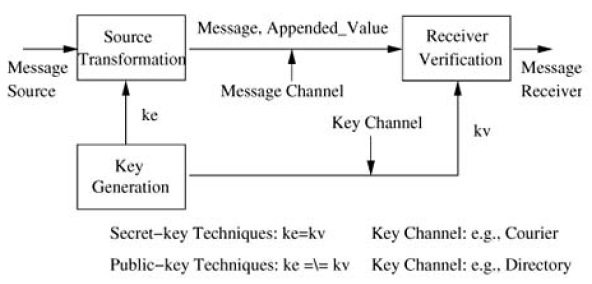
\includegraphics[scale=.4]{DataIntegrity}

\subsection*{Symmetric Techniques of Data Integrity}
A MDC is another term for a Message Authentication Code (MAC). A Mac can be created an verified using a keyed hash function technique, or using a block cipher encryption algorithm.
\subsubsection*{Cryptographic Hash Functions}
A Hash function is a deterministic function which maps a bit string of an arbitrary length to a hashed value which is a vit string of a fixed length.

\subsubsection*{Properties of a Hash Function}
\begin{itemize}
    \item Mixing-transformation\\
        On any input x, the output hashed value h(x) should be computationally indistinguishable from a uniform binary string.
    \item Collision Resistance\\
        It should be computationally infeasible to find two inputs x,y with \(x \neq y\) such that \(h(x)=h(y)\)
    \item Pre-image resistance\\
        Given a hashed value h, it should be computationally infeasible to find an input string such that \(h=h(x)\)
    \item Practical efficiency\\
        Given input string x, the computation of \(h(x)\) can be done in time bounded by a small-degree polynomial (ideally linear)
\end{itemize}

\subsubsection*{Hash Function Applications}
\begin{itemize}
    \item In digital signatures, hash functions are generally used for generating "message digests" or "message fingerprints."
    \item In public-key cryptosystems, has functions are widely used for realizing a cipher text correctness verification mechanism. This is necessary to protect an encryption scheme from active attackers.
    \item Hash Functions are used in wide range of applications, pseudo-randomness is required.
\end{itemize}

\subsubsection*{Random Oracle}
A Random Oracle is a very powerful and imaginary function that occurs if on any input, the distribution of the output hashed value is uniform.

\subsubsection*{Birthday Attack}
Assuming a hash function behaves as a random oracle, the square-root attack (birthday attack) suggests that,
\[2^{|h|/2}=\sqrt{2^{|h|}}\]
random evaluations of the hash function will suffice an attacker to obtain a collision with a non-negligible probablility. To mount the attack, the attacker should generate random message-hash pairs.
\[(m_{1},h(m_{1})),(m_{2},h(m_{2})), \ldots\]
until he ends up with finding two messages m and m' satisfying,
\[m \neq m',\texttt{ } h(m)=h(m')\]
This is only really usefull if the hashed message contains a meaningful sub-message.

\subsubsection*{MAC based Keyed Hash Function}
In a shared-key scenario a hash function takes a key as part of its input.
\[\texttt{MAC}=h(k \| M)\]
Where k is a secret key shared between the transmitter and receiver. \((\| = \texttt{concatenation})\)\\
The receiver should then recalculate the MAC from the message. If they match, then the message is believed to have come from the transmitter. In order for the receiver to verify itself to the sender, we must compute the HMAC,
\[\texttt{HMAC}=h(k \| M \| k)\]

\subsubsection*{MAC based on Block Cipher Encryption}
Let \(E_{k}(m)\) denote a block cipher encryption algorithm keyed with the key, k, on the input message, m. In order to authenticate a message, M, we need to divide M.
\[M = m_{1}m_{2}\ldots m_{l}\]
Where each sub-message block \(m_{i}, i=1,2,\dots,l\) has the size of the input of the block cipher algorithm. Let \(C_{0}=IV\) be a random initializing vector. Here the transmitter applies the CBC encryption:
\[C_{i} \leftarrow E_{k}(m_{i} \oplus C_{i-1}), i=1,2,\ldots,l\]
Then pair,
\[(IV,C_{l})\]

\subsection*{Digital Signatures}
\subsubsection*{the RSA Signature Scheme}
\begin{itemize}
    \item Key setup\\
        The key setup is identical to that of standard RSA cryptosystems.
    \item Signature Generation\\
        To create a signature of message, m, Alice create,
        \[s = \texttt{Sign}_{e}(m) \leftarrow m^{e}(\texttt{mod }N)\]
    \item Signature Verification\\
        Let Bob be a verifier who knows that the public-key material (N,e) belongs to Alice. Given a message-signature pair (m,s), Bob's verification procedture is,
        \[\texttt{Verify}_{(N,d)}(m,s) = \texttt{True if } m \equiv s^{d}(\texttt{mod }N)\]
\end{itemize}

\subsubsection*{Non-repudiation}
Non-repudiation is basically the idea that if there is a single entity responsible for creating a digital signature, then it is easy to settle disputes over who has created the signature. No denial of connection with a message.

% todo begining of midterm 3 material
\subsubsection*{Entity Authentication}
Entity authentication is a communication process by which a principal establishes alively correspondence with a second principal whose cliamed identity should meet what is sought by the first.
\begin{itemize}
    \item Host-host type: for example upon a reboot the system must identify to a trusted server neccessary information (like trusted copy of OS, trusted clock setting, or 
trusted environment settings) Client-Server setting where one host requests certain services from the other server.
    \item User-Host type: Computer login via telnet/ssh (Authenticated through some password protocol) In serious cases mutual authentication is required.
    \item Process-host type: used more for distributed computing. Ex) used for "mobile code" or a "browser based" java applet.
    \item Member-club type: ex a member of a club showing a membership card for access. Zero-knowledge identification protocols and undeniable signature schemes
\end{itemize}

\subsubsection{Manipulation Detection Code (MDC)}
\subsubsection*{Lively correspondence}
\begin{itemize}
    \item Freshness
        \begin{itemize}
            \item Freshness verifies that a message was sent sufficiently recently
            \item Data origin doesn't guarantee freshness.
            \item This prevents attacks that involve doing large computations on a message or replay attacks.
        \end{itemize}
    \item nonces
        \begin{itemize}
            \item A random number, used for verifying a challenge response.
            \item Simple example: bob sends a nonce to alice. Alice responds with the encrypted nonce, which was encrypted with a shared private key. If bob recieves the encrypted nonce (in a sufficiently short amount of time) and establishes it was encrypted correctly. This does not provide a proper data-integrity service.
        \end{itemize}
    \item timestamps
\end{itemize}

\subsubsection*{Data Origin Authentication}
\begin{itemize}
    \item Consists of transmitting a message from a purported source (the transmitter) to a receiver who will validate the message upon reception.
    \item The message validation conducted by the receiver aims to establish the identity of the message transmitter.
    \item The validation also aims to establish the data integrity of the message subsequent to its departure from the transmitter.
    \item The validation further aims to establish liveness of the the message transmitter.
\end{itemize}

\subsubsection*{Authentication vs Key exchange}
\begin{itemize}
    \item Key exchange or key agreement is usually used during entity authentation or as a subtask
\end{itemize}

\subsubsection*{Challenge-response}
\begin{itemize}
    \item Standard vs non-standard (encryption-then-decryption) challenge-response mechanisms
    \item Standard (as set by ISO, International Organization for Standardization and the IEC, International Electrotechnical Commission) of three challenge-response 
system.
\end{itemize}

\subsubsection*{Unilateral Authentication}
\begin{itemize}
    \item Only one of the two participants is authenticated.
\end{itemize}

\subsubsection*{Mutual authentication vs trusted third-party authentication}
\begin{itemize}
    \item In mutual authentication, both communicating entities are authenticated to each other.
    \item Originally simply unilateral authentication done twice, once in each direction, until wiener's attack (the Canadian Attack)
    \item Trusted Third Party (TTP) Authentication requires the principals to use a centralized open system from a trusted third party to authenticate.
\end{itemize}

\subsubsection*{Needham-Schroeder password protocol}
% todo expand on this
\begin{itemize}
    \item Premise: User, U and Host, H have setup U's password entry (\(ID_{u},f(P*u)\)) where f is a one-way function; U memorizes password \(P_u\)
    \item Goal: U logs in H using her/his password.
\end{itemize}
\begin{enumerate}
    \item U \(\rightarrow\) H : \(ID_u\);
    \item H \(\rightarrow\) U : "Input password:";
    \item U \(\rightarrow\) H : \(P_u\);
    \item H applies f on \(P_u\), finds entry (\(ID_u,f(P_u)\)) from its archive; Access is granted if the computed \(f(P_uP)\) matches the archived. Where f is a trapdoor function. In the unix password system, f is a series of 25 rounds of DES. Salt (12 bit random number) is used to randomize the flips.
\end{enumerate}
\begin{itemize}
    \item Data integrity of the password storage file becomes important and the protocol is still vulnerable to online password eavesdropping attack.
    \item One-time password scheme. In this flawed modification the number of times the hashing function is iterated one more time.
\end{itemize}

\subsection*{Passwords and salt}
\subsubsection*{Encryted key exchange (EKE)}
\begin{itemize}
    \item The EKE protocol protects the password against online eavesdropping and offline dictionary attacks.
    \item Premise: User, U and Host, H share a password \(P_u\); The system has agreed on a symmetric encryption algorithm, K() denotes symmetric encryption keyed by K; U and H also agreed on an asymmetric encryption scheme, \(E_u\) denotes asymmetric encryption under U's key.
    \item Goal: U and H achieve mutual entity authentication, they also agree on a shared secret key.
\end{itemize}
\begin{enumerate}
    \item U generates a random "public" key \(E_u\), and sends to H: U, \(P_u(E_u)\)
    \item H decrypts the cipher chunk using \(P_u\) and retrieces \(E_u\); H generates random symmetric key, K, and sends to U: \(P_u(E_u(K))\)
    \item U decrypts the doubly encrypted cipher chunk and obtains K; U generates a nonce \(N_u\), and sends to H: \(K(N_e)\)
    \item H decrypts the cipher chunk using K, generate a nonce, \(N_H\), and sends to U: \(K(N_u,N_h)\)
    \item U decrypts the cipher chunk using K, and return to H: \(K(N_h)\)
    \item If the challenge-response in 3,4,5 is successful, logging-in is granted and the parties proceed further secure communication
\end{enumerate}

\subsection*{Attacks on authentication protocols}
\subsubsection*{message replay attack}
\begin{itemize}
    \item Malice has previously recorded an old message from a previous run of a protocol and now replays the recorded message in a new run of the protocol
    \item blocked by freshness
\end{itemize}

\subsubsection*{man-in-the-middle attack}
Malice intercepts messages between Bob and Alice

\subsubsection*{parallel session attack}
The parallel session attack consists of two or more runs of a protocol executed concurrently under Malice's protection

\subsubsection*{relection attack}
A reflection attack is when an honest principal sends a message to an intended communication partner. Malice intercepts the message and reflects it back at the host

\subsubsection*{interleaving attack}
In an interleaving attack, two or more runs of a protocol are executed in an overlapping fashion under Malic's orchestration. Malic may compose a message and send it out to a principal in one run from which he expects to receive and answer.

\subsubsection*{attack due to type flaw}
Malice uses a flaw, including a principal being tricked to misinterpret a nonce, a timestamp or an indentification into key

\subsubsection*{attack due to name omission}
Name omission is a serious problem that could allow exploits

\subsubsection*{Kerberos}
\begin{itemize}
    \item single signon
        \begin{itemize}
            \item Each user memorizes a password, this is the single-signon credential for using the Kerberos system.
        \end{itemize}
    \item exchanges (authentication service exchange, ticket-granting service exchange, client-server authentication application exchange)
        \begin{itemize}
            \item Authentication Service Exchange (AS Exchange): runs between a client, C and an "authentication server", AS
            \item Ticket-Granting Service Exchange (TGS Exchange): runs between C and a "ticket granting server" TGS after the AS Exchange
                \begin{itemize}
                    \item Checks to see if the difference in time between the client time and host time are within a reasonable range for freshness.
                \end{itemize}
            \item Client/Server Authentication Application Exchange (AP Exchange): runs between C and an application server, S after the TGS Exchange
                \begin{itemize}
                    \item The AP Exchange a client, C that uses the newly obtained application session key, to obtain application services fromt he Application Servers
                \end{itemize}
        \end{itemize}
    \item key distribution center (authentication server, ticket granting server)
\end{itemize}

\subsubsection*{SSL/TLS}
\begin{itemize}
    \item Process: *=optional
\end{itemize}
\begin{enumerate}
    \item \(C \rightarrow S\): ClientHello
    \item \(S \rightarrow C\): Server Hello, ServerCertificate*, ServerKeyExchange*, CertificateRequest*, ServerHelloDone
    \item \(C \rightarrow S\): ClientCertificate*, ClientKeyExchange, CertificateVerify*, ClientFinished
    \item \(S \rightarrow C\): ServerFinished
\end{enumerate}
\begin{itemize}
    \item Hello Message Exchange: Server and Host let each other know what protocols they are capable of running
    \item handshake with key exchange
    \item crypto-suite selection, certificates
    \item use of nonces and random secrets
\end{itemize}


% You can even have references
\rule{0.3\linewidth}{0.25pt}
\scriptsize
\bibliographystyle{abstract}
\bibliography{refFile}
\end{multicols}
\end{document}
